
\makeatletter
\let\kernel@xfloat\@xfloat
\makeatother
\documentclass[12pt]{ksthesis}


\makeatletter
\let\@xfloat\kernel@xfloat
\def\@floatboxreset{%   
  \reset@font
  \linespread{1}\normalsize
  \@setminipage}
\makeatother   

\usepackage[cmex10]{amsmath}
%\usepackage{amsthm}
%\usepackage{amssymb}
%\usepackage{amsfonts}
\usepackage{graphicx}
%\usepackage{subfig}
\usepackage{subcaption}
%\usepackage{multirow}
\usepackage[ruled,vlined,linesnumbered]{algorithm2e}
%\usepackage{booktabs}
\usepackage{cite}
%\usepackage[utf8]{inputenc}
\usepackage{tabularx,ragged2e,booktabs,caption}
\captionsetup[figure]{font=large, labelfont=normalsize} \captionsetup[table]{name=Table, labelsep=colon} \captionsetup[figure]{justification=centering}
\captionsetup[table]{font=large, labelfont=normalsize} \captionsetup[table]{name=Table, labelsep=colon} \captionsetup[figure]{justification=centering}
\captionsetup[table]{name=Table, labelsep=colon}
\captionsetup[figure]{justification=centering}
\usepackage{indentfirst}
%\usepackage{array}
\usepackage{float}
%\usepackage{makecell}
\usepackage[strings]{underscore}
\usepackage{multirow}

%\paperwidth=8.5in \paperheight=11in % letter paper
\paperwidth=21cm \paperheight=29.6cm % A4 paper
\usepackage[left=3.0cm, right=2.5cm, top=2.3cm, bottom=3.5cm]{geometry}


\doublespace
\title{National Cheng Kung University
     \\Department of Electrical Engineering
     \\Master Thesis}
\author{Sung-Ho Chang}
\phdthesis

\Thesisspace
\begin{document}

\begin{preliminary} %---------- Preliminary ----------%

\setcounter{page}{2} \large

%------------------------- Abstract -------------------------%

\begin{abstract}
\begin{center}{\Large\textbf{
Trajectory Planning for Mission Completion Time Reduction in UAV-Assisted Data Collection in Wireless Sensor Networks
\vspace{0.3cm}\\
}\vspace{0.4cm}
}\end{center}

\begin{center}{\large 
Bo-Syun Ke\vspace{0.2cm} \\ 
Department of Electrical Engineering \vspace{0.2cm}\\ 
National Cheng Kung University \\
}\end{center}

\Thesisspace{\large 
	
    Unmanned aerial vehicles (UAVs) provide a flexible solution for data collection in wireless sensor networks (WSNs), especially when ground nodes (GNs) are deployed in wide or hard-to-access areas. Mission completion time (MCT) is an important performance metric in UAV-assisted data collection tasks. Existing studies have mainly focused on UAV flight trajectory planning to reduce mission completion time. But the data collection process also has a significant impact on MCT because the transmission rate varies with the distance between the UAV and GNs. 
    
    This thesis proposes a trajectory planning method for a single-UAV-assisted WSN data collection task. The proposed method first obtains a shortest geometric reference path that passes through the GN communication regions and uses this path as global directional guidance for local trajectory planning. For each GN, the UAV adjusts its data collection trajectory according to the required data amount. For adjacent GNs with overlapping communication regions, the proposed method further allows service switching within the overlap region to enable a more efficient transition to the next GN. Simulation results show that the proposed method outperforms the representative benchmark methods.
	
}

\emph{\textbf{Keywords}}---UAV, mission completion time, wireless sensor networks, trajectory planning, data collection.

\end{abstract}

%------------------------- Acknowledgement -------------------------%
%------------------------- Acknowledgement -------------------------%

\begin{acknowledgements}

\Thesisspace{\large

	First and foremost, I would like to express my deepest gratitude to my advisor, Professor Kuo-Feng Ssu, for his guidance, encouragement, and support throughout my academic journey at National Cheng Kung University. His invaluable advice and continuous support greatly contributed to the completion of this thesis. I would also like to thank Professors Hewijin Christine Jiau and Chia-Hung Kao for their valuable suggestions and for serving as members of my thesis committee. Their comments and feedback have helped improve the quality of this research. My sincere thanks also go to the members of the Dependable Computing Laboratory, including Yu-Jung Chang, Su Wu, You-Yao Chen, Hao-Chen Liu, Yen-Wei Lin, Xing-Ya Yang, Yu-Wei Zheng, Yun-Gung Chung, Zih-Yun Lin, Tzu-Hau Chen, and Yin-Wei Chiu, for their helpful advice, discussions, and support during my research. Finally, I am deeply grateful to my family and friends for their constant support, companionship, and encouragement. Their understanding and encouragement have given me the strength to complete this thesis.

}
\end{acknowledgements}


%------------------------- Content Table, List -------------------------%

\tableofcontents 
\listoffigures 
\listoftables 
\clearpage

\end{preliminary} %---------- Preliminary ----------%


\begin{thesis}\large{

%------------------------- Introduction -------------------------%
\chapter{Introduction}

    With the rapid development of the Internet of Things (IoT) and wireless communication technologies, wireless sensor networks (WSNs) have been widely applied in environmental monitoring, smart agriculture, post-disaster detection, military reconnaissance, and other fields~\cite{Qin2019, Zhang2023, Xiang2023UAVMEC}. In these applications, ground nodes (GNs) are mainly responsible for collecting environmental parameters, such as temperature, humidity, air quality, and water quality. In such IoT applications, each GN usually generates lightweight data packets~\cite{Meng2025UAVPathPlanningSurvey, Wei2022UAVIoTSurvey}. However, due to limited battery capacity and hardware cost, GNs are often unable to support long-distance wireless transmission. Therefore, transmitting sensing data back to a data center remains a major challenge.
    
    Unmanned aerial vehicles (UAVs) have become a feasible solution to this problem because of their high mobility, flexible deployment, and ability to establish favorable air-to-ground (A2G) line-of-sight (LoS) communication links~\cite{Zeng2019UAVTutorial, AlHourani2014LAPAltitude}. A UAV can serve as an aerial mobile data collector by actively approaching GNs and collecting data within their communication regions. This approach not only reduces the transmission power consumption of GNs and extends the lifetime of sensing devices, but also alleviates communication interruptions caused by terrain blockage~\cite{Zeng2019EnergyMinimization, Wu2018MultiUAVTrajectoryCommunication}.

    In UAV-assisted data collection tasks, mission completion time (MCT) is a critical performance metric~\cite{Zhang2023CompletionTimeDRL}. MCT refers to the total time required for the UAV to depart from the data center, complete data collection from all target GNs, and return to the data center. For time-sensitive IoT applications, such as real-time forest fire monitoring and border intrusion detection, reducing MCT allows the decision center to obtain on-site information more quickly and respond in a timely manner~\cite{Shen2022MultiUAVTimeWindows, Li2022MCT}. A shorter MCT also enables the UAV to serve more GNs within its limited battery~\cite{Li2023DataCollectionMaximization}. Early studies often approximated MCT by the UAV flight time and simplified the problem into a flight distance reduction problem~\cite{Alemayehu2017TSPHeuristic}. However, when communication models and data requirements are considered, a shortest geometric path does not necessarily lead to a shorter MCT~\cite{Gong2018FlightTimeMinimization, Fu2024CollectionPoint}. According to the Shannon formula, the wireless transmission rate increases with the signal-to-noise ratio (SNR), while the SNR decreases as the communication distance between the UAV and a GN increases~\cite{Wang2022TrajectoryPower}. If the UAV passes near the boundary of a GN communication region to reduce flight distance, the flight time can be shortened, but the lower transmission rate can increase the data collection time or hovering time. In contrast, if the UAV moves excessively close to the GN center to improve the transmission rate, additional flight distance and flight time can be introduced. Therefore, reducing MCT requires a proper tradeoff between flight distance and data collection time.

    Since the UAV only needs to enter the communication region of each GN to collect data and does not have to fly directly above every GN, this task can be regarded as a path planning problem with neighborhoods, namely the Traveling Salesman Problem with Neighborhoods (TSPN)~\cite{Luo2021TrajectoryWSN}. However, unlike conventional TSPN, which mainly focuses on geometric path length, UAV-assisted data collection is also affected by communication distance, transmission rate, and data collection time. Therefore, the UAV needs to determine not only the visiting path among communication regions, but also the entry position, exit position, movement depth, and data collection trajectory within each communication region. Existing studies have investigated UAV-assisted WSN data collection from different perspectives. Some studies reduce the geometric path length through GN communication regions~\cite{Luo2021TrajectoryWSN}, while other studies consider flying mode, hovering mode, or V-shaped collection trajectories~\cite{Wang2020CollaborativeUAVs, He2024VShapedTrajectory}. These studies show that MCT is affected by both flight time and data collection time. Two issues still require further consideration. First, if global geometric direction information is not considered, local trajectory adjustment can deviate from the overall shorter flight path. Second, when adjacent GN communication regions overlap, restricting service switching to the boundary of a single communication circle can cause redundant boundary transitions and unnecessary back-and-forth movement.

    Based on the above observations, this thesis focuses on a single-UAV-assisted WSN data collection task and proposes a trajectory planning method that considers both flight path and data collection efficiency. The proposed method combines global geometric information and a local data collection strategy to reduce the overall MCT of the UAV data collection task. The related mechanisms and implementation details are presented in the following chapters.

    \newpage
    The main contributions of this thesis are summarized as follows.

    \begin{enumerate}
    	\item A trajectory planning method is developed to reduce the MCT of UAV-assisted WSN data collection by considering both flight trajectory and data collection trajectory.
    	\item A global-direction-guided local trajectory adjustment method is introduced to keep local service trajectories close to the shortest geometric path and reduce unnecessary flight distance.
    	\item A flexible service switching strategy is developed for consecutive GNs with overlapping communication ranges, allowing the UAV to use shared coverage regions as switching areas and reduce redundant boundary transitions.
        \item Simulation results show that the proposed method reduces the overall MCT compared with the benchmark methods under different data requirements and GN distributions. 
    \end{enumerate}

    The remainder of this thesis is organized as follows. Chapter 2 reviews related studies on trajectory planning for UAV-assisted WSN data collection. Chapter 3 introduces the system model. Chapter 4 describes the proposed trajectory planning method. Chapter 5 presents the simulation setup, and performance evaluation. Finally, Chapter 6 concludes this thesis and discusses possible future research directions.

%------------------------- Related Works -------------------------%
\chapter{Related Work}\label{Chap:Related}
    
    In UAV-assisted WSN data collection tasks, existing studies can be broadly divided into two categories. The first category focuses on geometric path planning, where the communication range of each GN is regarded as a serviceable region, and the UAV flight path passing through all communication regions is shortened to reduce flight time. The second category considers the data collection process within the communication range, where the UAV adjusts its collection trajectory according to the required data amount and communication conditions. The former provides a shorter geometric reference path, whereas the latter reduces the data collection time.

    The study in~\cite{Luo2021TrajectoryWSN} modeled UAV path planning as a TSPN problem and showed that this problem is NP-hard. In~\cite{Li2020JointOptimization} considered a single-UAV-assisted data collection problem by jointly considering trajectory, altitude, velocity, and link scheduling. The study indicated that data transmission can be supported when the UAV is located within the communication range of a ground user, without requiring the UAV to fly directly above the ground user. The original mission time problem was transformed into a trajectory length problem. This method mainly focuses on shortening the geometric path length.

    Reference~\cite{Gong2018FlightTimeMinimization} indicated that simply shortening the flight distance can move the UAV farther away from sensor nodes, thereby reducing the transmission rate and increasing the time required to complete data reception. The results show that the flight distance, flight speed, and communication rate in UAV data collection tasks are not independent and should be considered jointly. The effect of the collection point location on mission time was further discussed in~\cite{Fu2024CollectionPoint}, where it was shown that the UAV data collection point should not be determined solely by the shortest flight distance or the best communication quality. If the UAV flies directly above a node, better communication quality can be achieved, but the flight distance can increase. In contrast, if the UAV collects data near the boundary of the communication range, the flight path can be shortened, but the longer distance between the UAV and the node reduces the transmission rate and increases the data collection time. This observation suggests that the collection point location should be determined by jointly considering the flight cost and the communication condition.

    In~\cite{Wang2020CollaborativeUAVs}, FM and HM were introduced as two data collection modes for UAVs. In FM, the UAV can continuously receive data while flying, which is suitable for nodes with smaller data requirements or better communication conditions. In HM, the UAV hovers at a specific location for data collection, which is suitable for nodes with larger data requirements or poorer communication conditions. The distinction between FM and HM allows the UAV to adjust its collection mode according to the node status and data requirement, instead of serving all nodes with a fixed collection mode.

    For user scheduling and UAV trajectory design,~\cite{Yuan2023CompletionTime} investigated the completion time problem for a single UAV collecting data from multiple sensor nodes. It was proved that, under specific conditions, a suitable UAV trajectory has an SHF structure, in which the UAV hovers at selected locations for data collection and flies at the maximum speed between these hovering locations. The authors also emphasized the importance of segment-based scheduling, meaning that the UAV mainly serves a specific sensor during a particular flying or hovering segment instead of frequently switching among different sensors.

    In~\cite{Li2022MCT} further investigated the impact of the data collection trajectory on the MCT and proposed a V-shaped collection trajectory. If the UAV flies into the interior of the communication range, part of the flight distance increases, but the SNR and transmission rate can be improved, thereby reducing the data collection time and the overall mission time. The work also pointed out that the service trajectories of adjacent nodes are coupled. The previous node affects the starting position when the UAV serves the next node. Therefore, if the service trajectory of each node is determined independently, additional flight distance can be introduced for subsequent nodes. In other words, locally reducing the data collection time of one node does not necessarily reduce the overall MCT. The UAV still needs to consider the continuous flight direction and service connection between adjacent nodes.

    The above studies show that trajectory planning for UAV-assisted data collection mainly involves two interrelated design aspects. First, geometric path planning methods reduce the flight distance for the UAV to pass through multiple communication regions~\cite{Luo2021TrajectoryWSN, Li2020JointOptimization}. Second, data collection trajectory design indicates that the UAV can moderately move into the communication range according to the required data amount and communication conditions, thereby improving the transmission rate and reducing the data collection time~\cite{Li2022MCT, Fu2024CollectionPoint}. In addition, existing studies have explained the close relationship between UAV flight behavior and communication conditions from the perspectives of flight speed and transmit power control, as well as FM/HM mode switching~\cite{Gong2018FlightTimeMinimization, Wang2020CollaborativeUAVs, Yuan2023CompletionTime}.

    Based on the above research context, this thesis focuses on a single-UAV-assisted WSN data collection task and investigates how to jointly consider the flight trajectory, the data collection trajectory within the communication range, and the service connection between adjacent nodes. Existing studies have shown the importance of geometric path shortening and data collection within the communication range. If trajectory planning mainly relies on geometric path length, the effect of the distance variation between the UAV and the GN on the data collection time cannot be fully reflected. In contrast, if the local data collection trajectory lacks a global geometric direction reference, the trajectory can gradually deviate from the shorter overall flight direction. In addition, when the communication ranges of adjacent or consecutive nodes overlap, the overlapping region provides additional flexibility for service switching. Effectively using this geometric property can help reduce unnecessary boundary switching and back-and-forth flight. Therefore, this study focuses on maintaining a shorter overall flight distance while considering the data collection efficiency within the communication range, and further utilizes the overlapping regions between adjacent communication ranges to improve service switching flexibility, thereby reducing the overall MCT.

%------------------------- Problem Formulation -------------------------%
\chapter{System Model}\label{Chap:Problem Formulation}

\section{System Model}

    As shown in Fig.~\ref{fig:system_model}, this thesis considers a UAV-assisted wireless sensor network in which a single UAV is employed to collect data from multiple ground nodes (GNs). The UAV departs from the data center, visits the communication regions of the GNs to collect their data, and returns to the data center after completing the data collection task. Let \(\mathcal{N}=\{g_1,g_2,\ldots,g_n\}\) denote the set of GNs, where \(n\) is the number of GNs. A three-dimensional Cartesian coordinate system is adopted, where the GNs are located on the ground plane and the UAV flies at a fixed altitude \(H\). The elevation angle between the UAV and a GN is denoted by \(\theta\), and the maximum flying speed of the UAV is denoted by \(v_{\max}\).
    
    During the data collection process, the UAV may operate in flying mode (FM) or hovering mode (HM). In FM, the UAV collects data while moving within the communication region of a GN. In HM, if the data collected along the flying trajectory is insufficient, the UAV hovers directly above the corresponding GN for additional data collection.
    
    \begin{figure*}[!t]
		\centering
		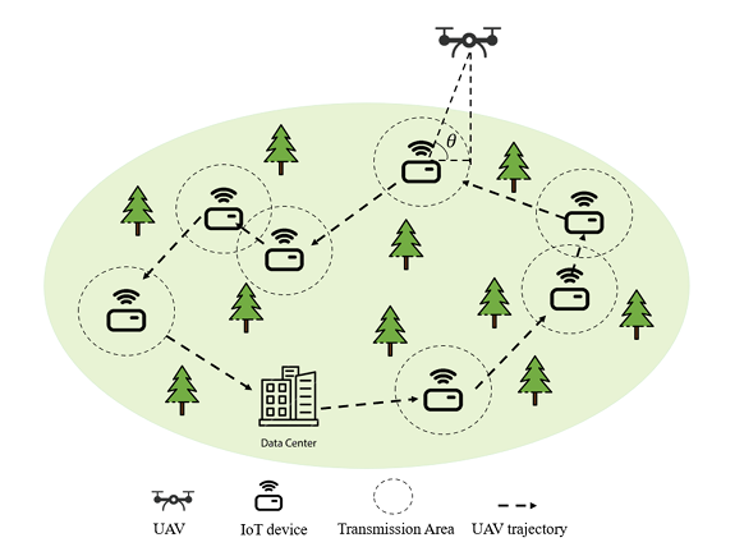
\includegraphics[width=1\textwidth]{./figures/system_model.png}
		\caption{Illustration of the UAV data collection process.} 
		\label{fig:system_model}
	\end{figure*}

    \noindent\textit{1) Transmission Model:} A delay-tolerant UAV-assisted WSN is considered, in which each ground node \(g_i\) stores sensing data and uploads the data to the UAV when the UAV enters its communication region. Each ground node is equipped with a single omnidirectional antenna and transmits with a fixed power \(P_t\) over a channel bandwidth \(B\). The uplink transmission rate from GN \(g_i\) to the UAV at time \(t\) is expressed as
    
    \begin{equation}
        R_i(t)=B\log_2\left(1+\gamma_i(t)\right)
    \end{equation}
    in which \(\gamma_i(t)\) denotes the received signal-to-noise ratio (SNR) from GN \(g_i\) to the UAV at time \(t\). The SNR is given by
    \begin{equation}
        \gamma_i(t)=\frac{P_t}{\sigma^2 L_{dB_i}(t)}
    \end{equation}
    where \(\sigma^2\) denotes the noise power at the UAV receiver, and \(L_{dB_i}(t)\) represents the air-to-ground path loss between GN \(g_i\) and the UAV at time \(t\). The UAV can successfully collect data only when the received SNR satisfies \(\gamma_i(t)\geq\bar{\gamma}\). To avoid transmission interference among ground nodes, only the ground node being served is allowed to transmit data to the UAV during its corresponding service interval.


    \noindent\textit{2) Channel Model:} Considering that the mission completion time generally exceeds the channel coherence time and that the UAV position changes during the mission, a statistical channel model is adopted. The path loss from GN \(g_i\) to UAV can be expressed as
    \begin{equation}
        L_{dB_i}(t)=\left(\frac{4\pi f_c}{c}\right)^2 l_i^{\eta}\left[P_{\mathrm{LoS}_i}(t)\left(\xi_{\mathrm{LoS}}-\xi_{\mathrm{NLoS}}\right)+\xi_{\mathrm{NLoS}}\right]
    \end{equation}
    where \(f_c\) denotes the carrier frequency, \(c\) is the speed of light, and \(\eta\) is the path-loss exponent. The parameters \(\xi_{\mathrm{LoS}}\) and \(\xi_{\mathrm{NLoS}}\) represent the average additional path losses under LoS and NLoS propagation conditions, respectively. In addition, \(l_i(t)\) denotes the three-dimensional distance between GN \(g_i\) and the UAV, which is given by
    \begin{equation}
        l_i(t)=\sqrt{\left(U_x(t)-GN_{ix}\right)^2+\left(U_y(t)-GN_{iy}\right)^2+H^2}
    \end{equation}
    where \(\left(GN_{ix},GN_{iy}\right)\) is the horizontal coordinate of GN \(g_i\), \(\left(U_x(t),U_y(t)\right)\) is the horizontal coordinate of the UAV at time \(t\), and \(H\) is the fixed flying altitude of the UAV.
    
    The LoS probability between GN \(g_i\) and the UAV is modeled as
    \begin{equation}
        P_{\mathrm{LoS}_i}(t)=\frac{1}{1+\alpha \exp\left[-\beta\left(\theta_i(t)-\alpha\right)\right]}
    \end{equation}
    where \(\alpha\) and \(\beta\) are parameters determined by the propagation environment. The elevation angle from GN \(g_i\) to the UAV at time \(t\) is denoted by \(\theta_i(t)\), which is defined as
    \begin{equation}
        \theta_i(t)=\frac{180}{\pi}\arcsin\left(\frac{H}{l_i(t)}\right).
    \end{equation}

    According to this channel model, the path loss is affected by both the UAV--GN distance and the elevation angle. When the UAV moves closer to a GN, the three-dimensional distance decreases and the elevation angle increases, which generally improves the LoS probability and reduces the average path loss. Therefore, the UAV trajectory directly affects the received SNR and the corresponding data collection time.

\section{Problem Formulation}
    In the considered single-UAV data collection mission, all GNs must be served within one flight. The UAV starts from the data center, collects the required data from each GN, and returns to the data center. For a given transmit power \(P_t\), the communication radius of each GN is determined by the SNR threshold \(\bar{\gamma}\). Let \(D\) denote the maximum horizontal distance between the UAV and a GN such that the received SNR is equal to \(\bar{\gamma}\). When the UAV is located inside the communication region with radius \(D\), the received SNR is no less than the required threshold, and the UAV can successfully receive data from the corresponding GN. The value of \(D\) is obtained according to the adopted LoS-based air-to-ground channel model.
	
    \begin{figure*}[!t]
		\centering
		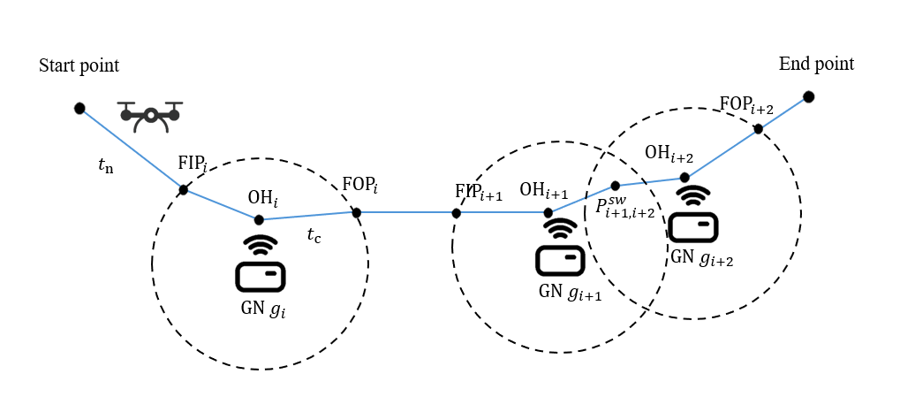
\includegraphics[width=1\textwidth]{./figures/uav_data_collection.png}
		\caption{UAV data collection process.} 
		\label{fig:uav_data_collection}
	\end{figure*}

    The MCT of the UAV is obtained by accumulating the service time required for all GNs. For each GN, the service time consists of the flight time required to reach its communication region and the data collection time spent within that region. The index \(i\) follows the service sequence along the UAV trajectory. The GN visiting sequence is first determined by a genetic algorithm (GA), and the proposed method plans the complete UAV trajectory based on this sequence. As shown in Fig.~\ref{fig:uav_data_collection}, GN \(g_i\) is served independently, whereas GN \(g_{i+1}\) and GN \(g_{i+2}\) share an overlapping communication region.
	
    UAV service trajectory is described by three key points: the flying-in point \(\mathrm{FIP}_i\), the optimal hovering or turning point \(\mathrm{OH}_i\), and the flying-out point \(\mathrm{FOP}_i\). The UAV first flies from the previous service point to \(\mathrm{FIP}_i\), and this flight duration is denoted by \(t_{n_i}\). After entering the communication region of GN \(g_i\), the UAV collects data while moving from \(\mathrm{FIP}_i\) to \(\mathrm{FOP}_i\) through \(\mathrm{OH}_i\). The corresponding data collection time is denoted by \(t_{c_i}\).

    When the communication regions of two consecutive GNs do not overlap, the UAV enters and leaves the communication region of each GN through its own FIP and FOP, respectively. In this case, \(\mathrm{FIP}_i\) and \(\mathrm{FOP}_i\) are located on the boundary of the communication region with radius \(D\), and the data collection trajectory of GN \(g_i\) is represented as
    \begin{equation}
        \mathrm{FIP}_i \rightarrow \mathrm{OH}_i \rightarrow \mathrm{FOP}_i.
    \end{equation}

    When the communication regions of GN \(g_{i+1}\) and GN \(g_{i+2}\) overlap, the service transition between the two GNs is represented by a common point selected from the overlapping region. Therefore, the FOP of GN \(g_{i+1}\) and the FIP of GN \(g_{i+2}\) are not forced to lie on the boundaries of their respective communication regions. To describe this service transition, this thesis introduces an overlap switching point, denoted by \(P^{\mathrm{sw}}_{i+1,i+2}\). The switching point satisfies
    \begin{equation}
        P^{\mathrm{sw}}_{i+1,i+2} \in D_{i+1} \cap D_{i+2}
    \end{equation}
    where \(D_i\) denotes the communication region of GN \(g_i\). The switching point simultaneously serves as the FOP of GN \(g_{i+1}\) and the FIP of GN \(g_{i+2}\), which is expressed as
    \begin{equation}
        \mathrm{FOP}_{i+1}=P^{\mathrm{sw}}_{i+1,i+2}=\mathrm{FIP}_{i+2}.
    \end{equation}

    The service trajectory across the overlapping communication regions of GN \(g_{i+1}\) and GN \(g_{i+2}\) can be represented as
    \begin{equation}
        \mathrm{FIP}_{i+1} \rightarrow \mathrm{OH}_{i+1} \rightarrow P^{\mathrm{sw}}_{i+1,i+2} \rightarrow \mathrm{OH}_{i+2} \rightarrow \mathrm{FOP}_{i+2}.
    \end{equation} 
    This representation indicates that the UAV completes the data collection of GN \(g_{i+1}\) before reaching the switching point, and then continues the data collection of GN \(g_{i+2}\) after passing through the same point. This setting keeps the trajectory continuous and allows the UAV to complete the service transition within the overlapping communication region, thereby avoiding unnecessary boundary departure and re-entry between consecutive GNs. For a group of consecutive overlapping GNs, the same concept is applied by defining an overlap switching point between each pair of adjacent GNs in the group.

    Except for hovering-based data collection, the UAV flies at the maximum speed \(v_{\max}\). Therefore, the flight time is proportional to the corresponding flight distance. For the flight segment from the previous service point to \(\mathrm{FIP}_i\), the flight time \(t_{n_i}\) is expressed as
    \begin{equation}
        t_{n_i}=\frac{d_{i1}}{v_{\max}}
    \end{equation}
    where
    \begin{equation}
        d_{i1}=\left\|\mathrm{FIP}_i-\mathrm{FOP}_{i-1}\right\|.
    \end{equation}

    For \(i=1\), \(\mathrm{FOP}_0\) denotes the data center. If GN \(g_i\) and the previously served GN overlap, \(\mathrm{FIP}_i\) can be the corresponding overlap switching point, and the fly-in distance is adjusted accordingly. After completing the data collection task of the last GN, the UAV returns to the data center. The return time is given by
    \begin{equation}
        t^r=\frac{\left\|\mathrm{DC}-\mathrm{FOP}_N\right\|}{v_{\max}}
    \end{equation}
    where \(\mathrm{DC}\) denotes the data center.

    The data collection time of GN \(g_i\), denoted by \(t_{c_i}\), is evaluated according to the adopted V-shaped collection trajectory. During this period, the UAV collects data while flying within the communication region. If the data collected during flight is insufficient, the UAV hovers directly above the corresponding GN to complete the remaining data collection. Let \(Q_i\) denote the required data amount of GN \(g_i\). The accumulated received data during the collection interval must satisfy
    \begin{equation}
        \int_{0}^{t_{c_i}} R_i(t)\,dt \geq Q_i.
    \end{equation}
    The MCT of the UAV is expressed as
    \begin{equation}
        T=\sum_{i=1}^{N}\left(t_{c_i}+t_{n_i}\right)+t^r.
    \end{equation}

    Let \(\mathcal{P}\) denote the set of service points associated with the UAV trajectory, including the FIPs, OHs, FOPs, and the overlap switching points when communication regions overlap. Based on the above definitions, the overall MCT reduction problem is formulated as
    \begin{equation}
    \begin{aligned}
    \textbf{(P1):}\quad 
    &\min_{U(t),\mathcal{P}}
    \left[
    \sum_{i=1}^{N}\left(t_{c_i}+t_{n_i}\right)+t^r
    \right] \\
    \text{s.t.}\quad 
    &\gamma_i(t)\geq \bar{\gamma} \\
    &\mathrm{FIP}_i,\mathrm{OH}_i,\mathrm{FOP}_i \in D_i \\
    &P^{\mathrm{sw}}_{i,i+1} \in D_i \cap D_{i+1},\ i\in \mathcal{O} \\
    &\int_{0}^{t_{c_i}} R_i(t)\,dt \geq Q_i
    \end{aligned}
    \end{equation}
    Here, \(\mathcal{O}\) denotes the set of consecutive GN indices whose communication regions overlap, i.e., \(D_i \cap D_{i+1} \neq \emptyset\). Constraint (17a) ensures that the received SNR satisfies the required threshold during data collection. Constraint (17b) requires the key service points of each GN to lie within the corresponding communication region. Constraint (17c) defines the feasible region of the overlap switching point. Constraint (17d) guarantees that the required data amount of each GN is collected.

    Problem \textbf{P1} is difficult to solve directly because the flight trajectory and the data collection trajectory are coupled. The selection of service points in \(\mathcal{P}\) affects both the flight time \(t_{n_i}\) and the data collection time \(t_{c_i}\). Moreover, when consecutive communication regions overlap, the overlap switching points affect the continuity of the service trajectory across adjacent GNs. Therefore, this thesis addresses \textbf{P1} through two trajectory planning components in the proposed solution: single-node trajectory planning and overlapping-node group trajectory planning. The RPA mechanism provides reference-path attractors for both components, whereas the BO strategy is specifically applied to overlapping-node groups to determine feasible service switching points within overlapping communication regions.

%------------------------- Proposed Solution -------------------------%
\chapter{Proposed Solution}\label{Chap:Proposed Solution}
	
    This chapter presents the proposed trajectory planning method for reducing the mission completion time (MCT) in UAV-assisted WSNs. Since the MCT is determined by both flight time and data collection time, a trajectory with the shortest geometric length does not necessarily lead to the shortest mission duration. Therefore, the proposed method is developed based on two design considerations: reducing both the flight distance and the data collection time of each GN.

    To achieve this objective, this thesis first constructs a shortest geometric reference path to provide global directional information. Based on this reference path, the Reference-Path Attractor (RPA) mechanism is used to guide the subsequent local trajectory planning process. The final UAV trajectory is then determined according to the data collection requirement of each GN and the spatial relationship among communication regions. Through this design, the UAV trajectory can remain close to the shortest geometric reference path while allowing the UAV to move deeper into the communication region when such movement can improve the transmission rate and reduce the data collection time.

    Based on the spatial relationship among GNs, the proposed trajectory planning process is divided into two cases. For an independent GN whose communication region does not overlap with the communication regions of other GNs, this thesis applies single-node trajectory planning to determine the corresponding service trajectory. For consecutive GNs with overlapping communication regions, this thesis adopts the Boundary-Overlap Strategy (BO), which treats the overlapping GNs as a group and uses the flexibility provided by the overlapping regions to determine the service trajectory.

    The remainder of this chapter is organized as follows. Section~5.1 introduces the construction of the shortest geometric reference path and the Reference-Path Attractor (RPA) mechanism. Section~5.2 presents the single-node trajectory planning method. Section~5.3 describes the overlapping-node group trajectory planning method based on BO.
    
\section{Reference Path Construction and RPA Mechanism}

    The purpose of constructing a shortest geometric reference path is to provide a global geometric direction for the subsequent trajectory planning process. If the trajectory segment associated with each GN is determined only according to the data collection time of the current GN, the selection of FIP and FOP may lack guidance from the shortest geometric reference path. As a result, the subsequent trajectory may deviate from the shortest geometric reference path, leading to an increase in flight distance. Therefore, this thesis first computes a shortest geometric reference path that passes through all GN communication regions and then extracts reference-path attractors from this path. In this thesis, an attractor is defined as a reference point extracted from the shortest geometric reference path within the communication region of a GN. The attractor is used as a directional reference when evaluating candidate FIP/FOP pairs in later trajectory planning, but the UAV is not required to pass through the attractor.

    Following the service order defined in the problem formulation, the index \(i\) denotes the \(i\)-th GN visited by the UAV, and the communication region of this GN is denoted by \(\mathcal{D}_i\), as defined in the system model. For the given visiting sequence, this thesis computes a shortest geometric path that passes through all communication regions \(\mathcal{D}_i\). To formulate the reference path construction problem, two auxiliary reference-path points are introduced for each communication region. Let \(\mathbf{r}_i^{\mathrm{in}}\) and \(\mathbf{r}_i^{\mathrm{out}}\) denote the reference-path entry point and reference-path exit point associated with \(\mathcal{D}_i\), respectively. These two points are used only for constructing the shortest geometric reference path and are not the final FIP and FOP used for data collection. The shortest geometric reference path is obtained by solving
    \begin{equation}
    \begin{aligned}
    \min_{\{\mathbf{r}_i^{\mathrm{in}},\mathbf{r}_i^{\mathrm{out}}\}_{i=1}^{N}} \quad
    & \left\|\mathbf{r}_1^{\mathrm{in}}-\mathbf{q}_0\right\|
    + \sum_{i=1}^{N}\left\|\mathbf{r}_i^{\mathrm{out}}-\mathbf{r}_i^{\mathrm{in}}\right\| \\
    &+ \sum_{i=1}^{N-1}\left\|\mathbf{r}_{i+1}^{\mathrm{in}}-\mathbf{r}_i^{\mathrm{out}}\right\|
    + \left\|\mathbf{q}_0-\mathbf{r}_N^{\mathrm{out}}\right\| \\
    \text{s.t.} \quad
    & \mathbf{r}_i^{\mathrm{in}} \in \mathcal{D}_i \\
    & \mathbf{r}_i^{\mathrm{out}} \in \mathcal{D}_i .
    \end{aligned}
    \end{equation}
    where \(\mathbf{q}_0\) denotes the data center. The first term represents the distance from the data center to the reference-path entry point of the first visited GN. The second term represents the geometric segment inside each communication region. The third term represents the distance from the reference-path exit point of the current GN to the reference-path entry point of the next visited GN. The last term represents the return distance from the last communication region to the data center. Since the objective function is composed of Euclidean norm terms and the feasible communication regions are convex, (5.1) can be formulated as a SOCP problem.

    The segment from \(\mathbf{r}_i^{\mathrm{in}}\) to \(\mathbf{r}_i^{\mathrm{out}}\) represents only the portion of the shortest geometric reference path inside the communication region \(\mathcal{D}_i\), rather than the actual data collection trajectory of the \(i\)-th GN. The final FIP, OH, and FOP are determined later according to the data requirement of the GN and the corresponding data collection time. Therefore, the shortest geometric reference path provides geometric reference information for the subsequent trajectory planning process.


    After the shortest geometric reference path is obtained, the RPA mechanism extracts one attractor for each GN. Let the shortest geometric reference path be denoted by \(\mathcal{P}_{\mathrm{ref}}\). The path \(\mathcal{P}_{\mathrm{ref}}\) is scanned according to the traveling direction from the data center. For the \(i\)-th GN, the candidate attractor points are the points on \(\mathcal{P}_{\mathrm{ref}}\) that lie within the communication region \(\mathcal{D}_i\). Let \(\ell(\mathbf{p})\) denote the cumulative path length from \(\mathbf{q}_0\) to point \(\mathbf{p}\) along \(\mathcal{P}_{\mathrm{ref}}\). The attractor of the \(i\)-th GN is defined as
    \begin{equation}
        \mathbf{a}_i=\operatorname*{arg\,min}_{\mathbf{p}\in\mathcal{P}_{\mathrm{ref}}\cap\mathcal{D}_i}\ell(\mathbf{p}).
    \end{equation}
    As shown in Fig.~\ref{fig:reference_path_attractors}, the shortest geometric path passes through the communication regions of the GNs according to the visiting direction. The triangular markers indicate the reference-path attractors extracted from this path. Each attractor is selected from the portion of the shortest geometric path that lies within the corresponding communication region.
    \begin{figure*}[!t]
		\centering
		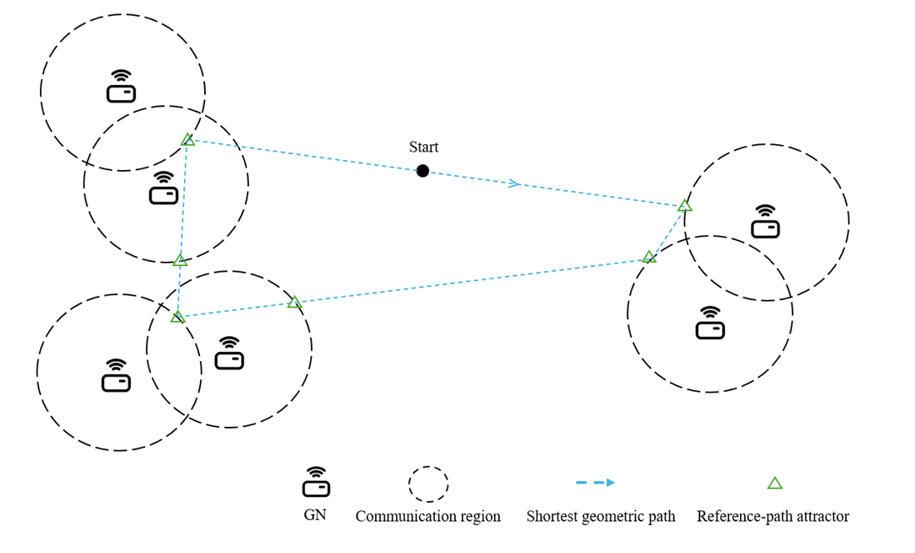
\includegraphics[width=1\textwidth]{./figures/reference_path_attractors.png}
		\caption{Illustration of the reference-path attractors.} 
		\label{fig:reference_path_attractors}
	\end{figure*}

    The attractor \(\mathbf{a}_i\) is selected as the first reference-path point that lies within the communication region of the \(i\)-th GN along the traveling direction. This early-entry selection preserves a longer available data collection interval along the reference path. Therefore, \(\mathbf{a}_i\) is used as the reference-path entry point associated with the \(i\)-th GN. The terminal attractor is set as the data center, \(\mathbf{a}_{N+1}=\mathbf{q}_0\).

    The influence of the attractor can be explained by decomposing the flight-time term associated with the \(i\)-th GN. Let \(\mathbf{P}_i^{\mathrm{pre}}\) denote the point immediately before serving the \(i\)-th GN. The point \(\mathbf{P}_i^{\mathrm{pre}}\) can be the FOP of the previous GN, an overlap switching point, or the data center when \(i=1\). For a candidate \(\mathrm{FIP}_i\), the fly-in time is expressed as
    \begin{equation}
        t_{n_i}^{\mathrm{in}}=\frac{\left\|\mathrm{FIP}_i-\mathbf{P}_i^{\mathrm{pre}}\right\|}{v_{\max}}.
    \end{equation}
    After the data collection process of the \(i\)-th GN is completed, the outgoing flight direction is evaluated with respect to the next attractor \(\mathbf{a}_{i+1}\). The RPA-guided fly-out time is expressed as
    \begin{equation}
        t_{n_i}^{\mathrm{out}}=\frac{\left\|\mathbf{a}_{i+1}-\mathrm{FOP}_i\right\|}{v_{\max}}.
    \end{equation}
    Accordingly, the flight-time term considered in the RPA-guided trajectory planning process is written as
    \begin{equation}
        t_{n_i}^{\mathrm{RPA}}=t_{n_i}^{\mathrm{in}}+t_{n_i}^{\mathrm{out}}.
    \end{equation}
    The fly-out term \(t_{n_i}^{\mathrm{out}}\) shows how the next attractor affects the evaluation of the current FOP. When different FIP/FOP pairs are considered in the trajectory evaluation process, the selected FOP determines the flight time toward the next attractor. Therefore, the RPA mechanism affects the selection of the FIP/FOP pair through the RPA-guided flight-time term.

    A candidate FIP/FOP pair is evaluated not only according to the data collection time of the current GN, but also according to the flight time toward the reference direction derived from the shortest geometric reference path. The UAV trajectory is not constrained to pass through the attractor. The complete candidate evaluation rule is described in Section~5.2.

    Algorithm~\ref{alg:rpa} summarizes the procedure for constructing the shortest geometric reference path and extracting the corresponding reference-path attractors. Based on the extracted attractors and the RPA-guided flight-time term, Section~5.2 presents the single-node trajectory planning method, including the generation of candidate FIP/FOP pairs, the determination of OH, and the evaluation of \(t_{c_i}\). Section~5.3 further describes how the trajectory planning process is modified when consecutive GNs have overlapping communication regions.

    \begin{algorithm}[H]
    \caption{Reference Path Construction and Attractor Extraction}
    \label{alg:rpa}
    \KwIn{Communication regions \(\{\mathcal{D}_i\}_{i=1}^{N}\) in the visiting order; data center \(\mathbf{q}_0\)}
    \KwOut{Shortest geometric reference path \(\mathcal{P}_{\mathrm{ref}}\); reference-path attractors \(\{\mathbf{a}_i\}_{i=1}^{N+1}\)}

    Solve the SOCP problem in \eqref{eq:reference-path-construction} to obtain \(\{\mathbf{r}_i^{\mathrm{in}},\mathbf{r}_i^{\mathrm{out}}\}_{i=1}^{N}\)\;

    Construct the shortest geometric reference path \(\mathcal{P}_{\mathrm{ref}}\):
    \[
    \mathcal{P}_{\mathrm{ref}}:
    \mathbf{q}_0
    \rightarrow
    \mathbf{r}_1^{\mathrm{in}}
    \rightarrow
    \mathbf{r}_1^{\mathrm{out}}
    \rightarrow
    \cdots
    \rightarrow
    \mathbf{r}_N^{\mathrm{in}}
    \rightarrow
    \mathbf{r}_N^{\mathrm{out}}
    \rightarrow
    \mathbf{q}_0 .
    \]

    Define \(\ell(\mathbf{p})\) as the cumulative path length from \(\mathbf{q}_0\) to point \(\mathbf{p}\) along \(\mathcal{P}_{\mathrm{ref}}\)\;

    \For{\(i=1\) \KwTo \(N\)}{
        Extract the first reference-path point that lies within \(\mathcal{D}_i\):
        \[
        \mathbf{a}_i
        =
        \operatorname*{arg\,min}_{\mathbf{p}\in \mathcal{P}_{\mathrm{ref}}\cap \mathcal{D}_i}
        \ell(\mathbf{p}).
        \]
    }

    Set the terminal attractor as the data center:
    \[
    \mathbf{a}_{N+1}=\mathbf{q}_0 .
    \]

    \Return \(\mathcal{P}_{\mathrm{ref}}\) and \(\{\mathbf{a}_i\}_{i=1}^{N+1}\)\;
    \end{algorithm}


\section{Single-Node Trajectory Planning}

    This section describes the trajectory planning process for an independent GN. An independent GN is defined as a GN whose communication region does not overlap with the communication regions of other GNs. Based on the RPA-guided flight-time term defined in Section~5.1, this planning process selects a suitable FIP/FOP pair while considering the data collection time inside the communication region. The corresponding OH is determined during the evaluation of the V-shaped data collection trajectory.

    \begin{figure*}[!t]
		\centering
		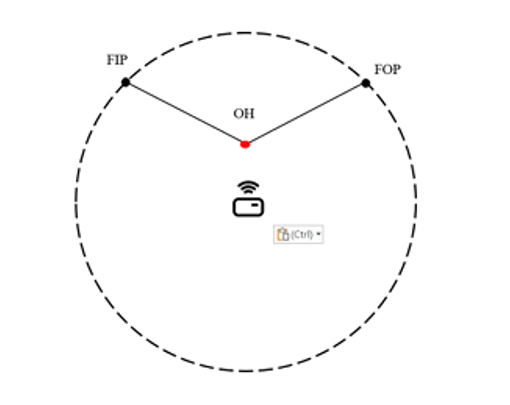
\includegraphics[width=0.7\textwidth]{./figures/single_node_data_collection.png}
		\caption{V-shaped trajectory for single-node data collection.} 
		\label{fig:single_node_data_collection}
	\end{figure*}

    As shown in Fig.~\ref{fig:single_node_data_collection}, the UAV collects data while moving inside the communication region of the GN. Candidate FIP and FOP points are generated on the communication boundary of the GN. Let \(\mathcal{F}_i^{\mathrm{in}}\) and \(\mathcal{F}_i^{\mathrm{out}}\) denote the candidate sets of FIP and FOP, respectively. For each candidate pair \((\mathrm{FIP}_i,\mathrm{FOP}_i)\), the corresponding \(\mathrm{OH}_i\) and the data collection time \(t_{c_i}\) are evaluated according to the required data amount \(C_i\).

    For each candidate pair, the corresponding V-shaped trajectory is evaluated to determine whether the required data amount can be collected during flight. If the flying collection is sufficient, FM is adopted. If the flying collection is insufficient, HM is adopted, and the UAV collects the remaining data by hovering. After the data collection time is obtained for all candidate pairs, the candidate pair is selected by considering both \(t_{c_i}\) and the RPA-guided flight-time term \(t_{n_i}^{\mathrm{RPA}}\).

    For a given FIP/FOP pair, the flying distance inside the communication region is determined by the sum of the distance from FIP to OH and the distance from OH to FOP. According to the geometric property of an ellipse, all points with the same sum of distances to \(\mathrm{FIP}_i\) and \(\mathrm{FOP}_i\) form an elliptical curve. Therefore, different V-shaped trajectories can be evaluated by adjusting \(\mathrm{OH}_i\) and the corresponding internal flying distance. When the required data amount can be collected during flight, a bisection search is used to determine a feasible V-shaped flying trajectory that satisfies the data collection requirement.
    
    The amount of data collected during flight is calculated by integrating the instantaneous transmission rate along the trajectory:
    \begin{equation}
        C_i^{\mathrm{FM}}=\int_{0}^{t_i^{\mathrm{FM}}} R_i(t)\,dt.
    \end{equation}
    where \(t_i^{\mathrm{FM}}\) denotes the flying collection time of the candidate V-shaped trajectory. If \(C_i^{\mathrm{FM}}\geq C_i\), the required data amount can be collected in FM, and the data collection time is given by \(t_{c_i}=t_i^{\mathrm{FM}}\). If \(C_i^{\mathrm{FM}}<C_i\), the flying trajectory cannot collect all required data. The UAV then operates in HM. In HM, OH is used as the hovering point, and the UAV collects the remaining data at this point. The additional hovering time is calculated as
    \begin{equation}
        t_i^{\mathrm{H}}=\frac{C_i-C_i^{\mathrm{FM}}}{R_i(\mathrm{OH}_i)}.
    \end{equation}
    Therefore, the data collection time in HM is
    \begin{equation}
        t_{c_i}=t_i^{\mathrm{FM}}+t_i^{\mathrm{H}}.
    \end{equation}
    After \(t_{c_i}\) is obtained for all candidate FIP/FOP pairs, each candidate is evaluated together with the RPA-guided flight-time term. The selected pair is determined by
    \begin{equation}
        \min_{\mathrm{FIP}_i,\mathrm{FOP}_i}
        \ t_{c_i}\left(\mathrm{FIP}_i,\mathrm{OH}_i,\mathrm{FOP}_i\right)
        + t_{n_i}^{\mathrm{RPA}} .
    \end{equation}

    In (5.12), \(\mathrm{OH}_i\) is determined during the evaluation of \(t_{c_i}\). Therefore, the selected pair is determined by considering both the data collection time inside the communication region and the RPA-guided flight time. After the trajectory of the current GN is determined, the resulting FOP is used as the starting point for planning the next GN. When consecutive GNs have overlapping communication regions, the corresponding overlapping-node trajectory planning method is described in Section~5.3.


\section{Overlapping-Node Group Trajectory Planning}
    This section describes the trajectory planning method for GNs with overlapping communication regions. For an independent GN, the FIP and FOP candidates are generated on the communication boundary of a single GN, as described in Section~5.2. When the communication regions of adjacent GNs overlap, the overlapping region provides additional flexibility for service transition. If the UAV is still forced to leave one communication region from its boundary and enter the next communication region from another boundary point, unnecessary flight distance may be introduced. 

    To use the overlapping region between adjacent GNs, this thesis proposes the Boundary-Overlap Strategy (BO). BO allows the switching point \(P^{\mathrm{sw}}_{i,i+1}\), defined in the system model, to be selected from the overlapping region of \(g_i\) and \(g_{i+1}\). In this way, the UAV can connect the service trajectory of two adjacent GNs through the overlapping region, instead of performing an additional boundary-to-boundary transition.

    \begin{figure*}[!t]
		\centering
		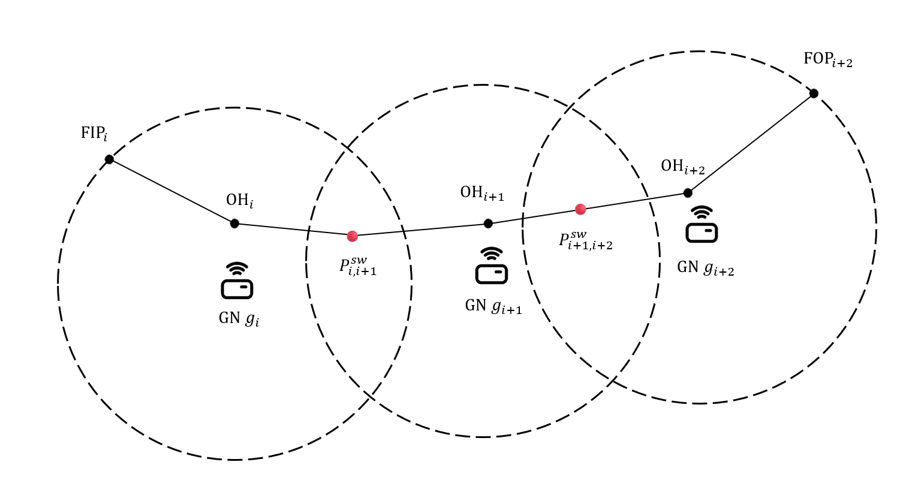
\includegraphics[width=0.9\textwidth]{./figures/overlap_trajectory.png}
		\caption{Boundary-Overlap Strategy for overlapping GNs.} 
		\label{fig:overlap_trajectory}
	\end{figure*}

    As shown in Fig.~\ref{fig:overlap_trajectory}, multiple adjacent GNs with overlapping communication regions are considered as one group. Let
    \begin{equation}
        G_m=\{g_i,g_{i+1},\ldots,g_j\}
    \end{equation}
    denote the \(m\)-th overlapping-node group, where \(g_i\) and \(g_j\) are the first and last GNs in the group, respectively. Here, \(G_m\) denotes a set of GNs, while \(g_i\) denotes an individual GN. For any two adjacent GNs \(g_k\) and \(g_{k+1}\) in \(G_m\), where \(k=i,\ldots,j-1\), their communication regions overlap. The UAV enters the group from the FIP of \(g_i\), passes through the switching points in the overlapping regions and leaves the group from the FOP of \(g_j\). For example, if the group contains \(g_i\), \(g_{i+1}\), and \(g_{i+2}\), the service trajectory inside the group can be represented as
    \begin{equation}
        \mathrm{FIP}_i
        \rightarrow
        \mathrm{OH}_i
        \rightarrow
        P^{\mathrm{sw}}_{i,i+1}
        \rightarrow
        \mathrm{OH}_{i+1}
        \rightarrow
        P^{\mathrm{sw}}_{i+1,i+2}
        \rightarrow
        \mathrm{OH}_{i+2}
        \rightarrow
        \mathrm{FOP}_{i+2}.
    \end{equation}
    In this sequence, \(\mathbf{P}^{\mathrm{sw}}_{i,i+1}\) is used as the exit point of \(g_i\) and the entry point of \(g_{i+1}\). Similarly, \(\mathbf{P}^{\mathrm{sw}}_{i+1,i+2}\) connects the service trajectories of \(g_{i+1}\) and \(g_{i+2}\). Therefore, the group is planned as a single service unit with one entry point and one exit point.

    For each overlapping region, BO selects the switching point from a finite candidate set instead of searching over the entire continuous overlapping region. The candidate set is generated using two representative sampling directions. The first direction follows the line segment connecting the centers of the two adjacent GNs. Since different adjacent GN pairs may have different overlap depths. Therefore BO can adjust whether the service transition should occur earlier or later within the overlapping region. The second direction follows a perpendicular sampling line inside the overlapping region. This direction provides candidates with different inward depths within the overlapping region. Since different data amounts may require different collection depths, the perpendicular sampling line allows BO to adjust the switching location according to the data collection requirement. By combining these two representative directions, the T-shaped sampling method generates switching candidates for the overlapping region without searching all possible points in the continuous region.

%------------------------- Performance Evaluation-------------------------%
\chapter{Performance Evaluation}\label{Chap:Implementation}

    The evaluation of the system was performed on Python 3.12.3 running on an AMD Ryzen 5 3600 CPU. A network comprising 100 nodes was generated using the Barabasi-Albert model~\cite{barabasi1999emergence}, with the average node degree configured to 5. The channel capacity for each channel was set using the data from bitcoinvisuals.com~\cite{BitcoinVisuals}. Channel transaction fees were generated based on the average fee values and median values provided by 1ml.com~\cite{1ML}. For transaction amounts, this study sampled credit card transaction amounts from the Credit Card Fraud Detection dataset~\cite{CreditCardFraudULB}. Transaction partner combinations were generated with the research data from Flash~\cite{Flash}. This approach aimed to simulate realistic transaction patterns. Regarding the simulator setup, this system employed Poisson distribution simulations to randomly generate transaction arrival times for various transaction frequencies (TPS). The single-hop latency in the experiment was set to 30 ms, referencing Deter-Pay~\cite{Deter-Pay}. Additionally, transactions were enabled to execute concurrently.

    \begin{table}[t]
      \caption{Simulation Parameters}
      \label{tab:params}
      \centering 
      \begin{tabular}{lc} 
        \toprule
        \textbf{Parameter} & \textbf{Value} \\
        \midrule
        Number of Nodes & 100 \\
        Number of Channels & 521 \\
        Average Channel Capacity & 8,929,583 satoshis \\
        Median Channel Capacity & 1,589,612 satoshis \\
        Transaction Frequency (TPS) & 10---100 \\
        Transaction Amount Range & 0.0---25,691.16 USD \\
        Simulation Duration & 30---60 s \\
        Single-hop Latency & 30 ms \\ 
        \bottomrule
      \end{tabular}
    \end{table}

\section{Comparison Algorithms}
    \begin{enumerate}
        \item \textbf{Shortest Path}: Shortest path routing is currently employed in the Lightning Network to determine the path between senders and receivers for payments.
        \item \textbf{Flash}~\cite{Flash}: Flash differentiates between high-value ???elephant??? payments and low-value ???mice??? payments. The strategy can improve success rates.
        \item \textbf{Deter-Pay}~\cite{Deter-Pay}: Deter-Pay combines precomputed candidate paths with a probing-based balance reservation mechanism.
    \end{enumerate}
\section{Performance Under Different Workloads}
  
    The experiment aims to verify the algorithm's comprehensive performance under varying transaction frequencies. The experimental setup configures the transaction frequency per second from 10 TPS to 100 TPS. The transaction success rate, execution time, and transaction fees incurred per satoshi are recorded with the varying frequencies.
    
    \begin{figure}[htbp]
        \centering
        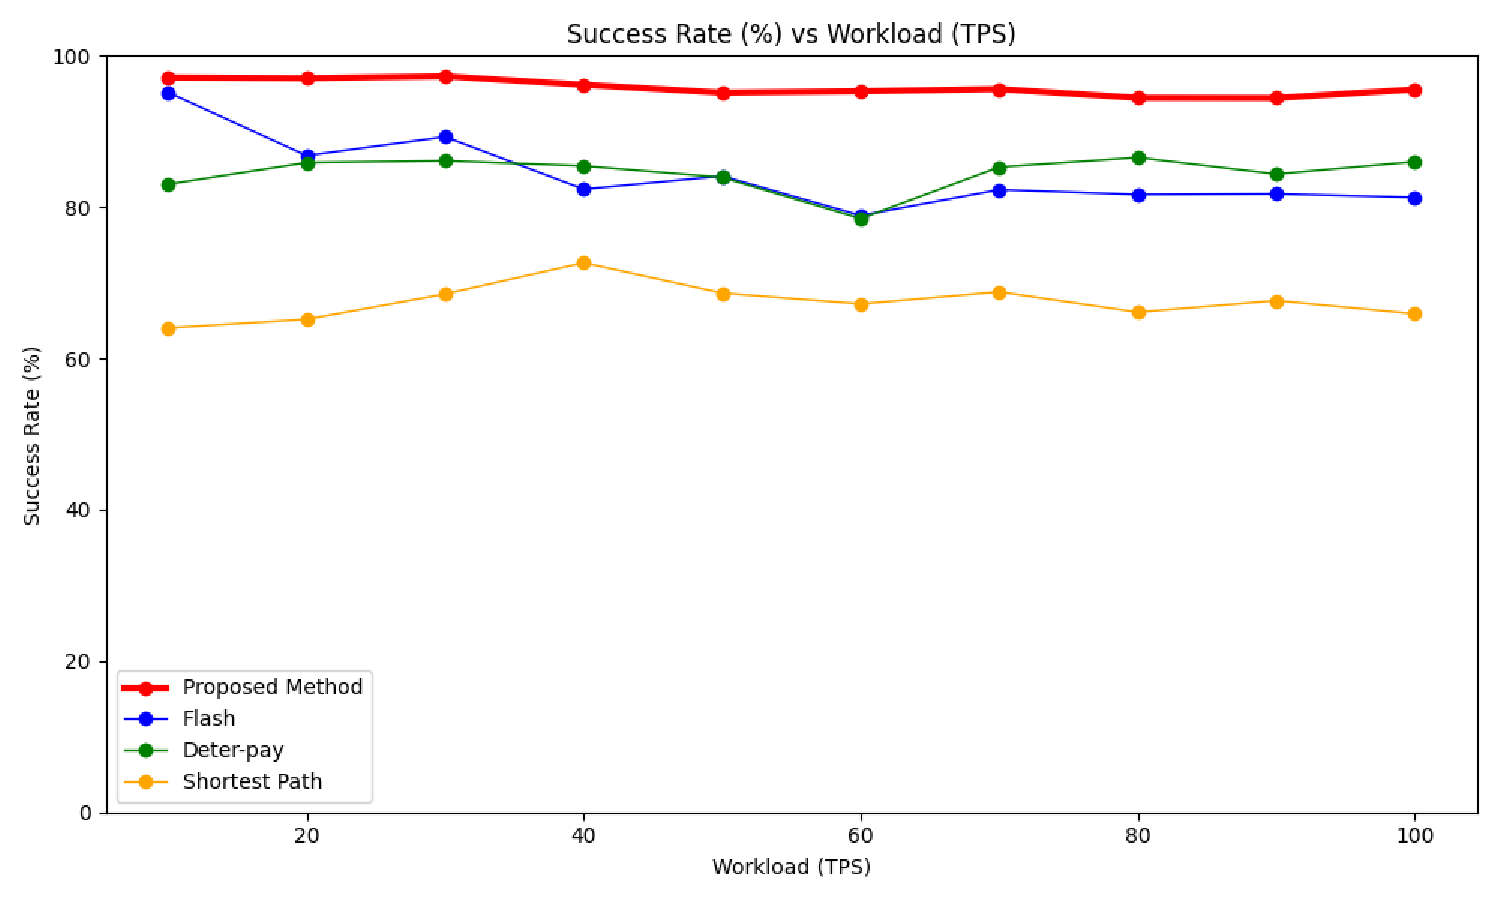
\includegraphics[width=\textwidth]{./figures/Success_rate.pdf}
        \caption{Success rate under different workloads.}
        \label{fig:Success_rate_TPS}
    \end{figure}
    
    \begin{figure}[htbp]
        \centering
        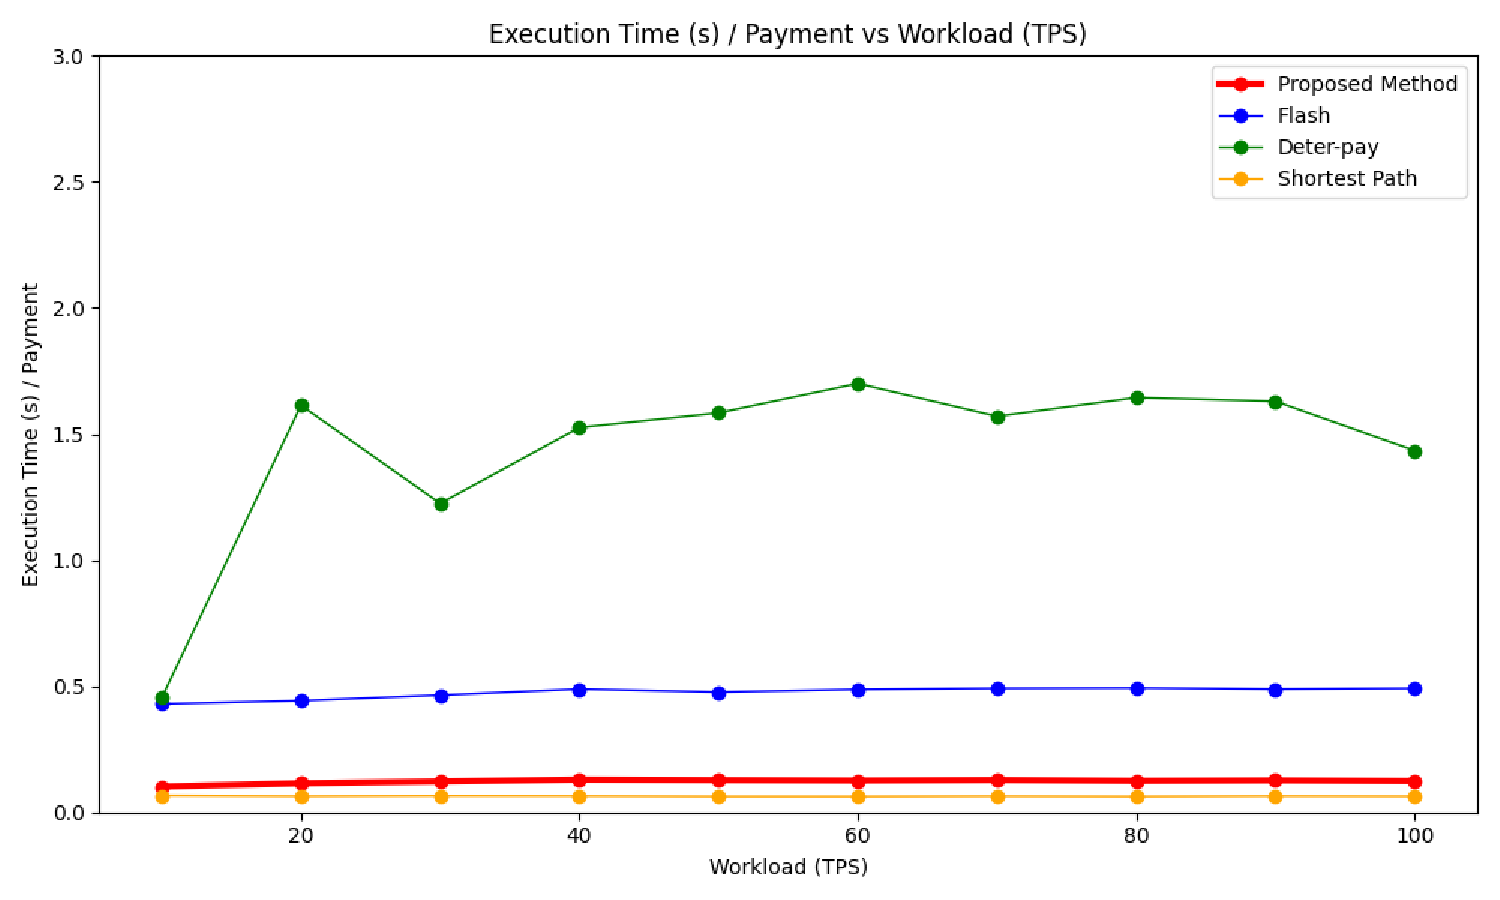
\includegraphics[width=\textwidth]{./figures/Excution_time.pdf}
        \caption{Execution time under different workloads.}
        \label{fig:Excution_time_TPS}
    \end{figure}
    
    \begin{figure}[htbp]
        \centering
        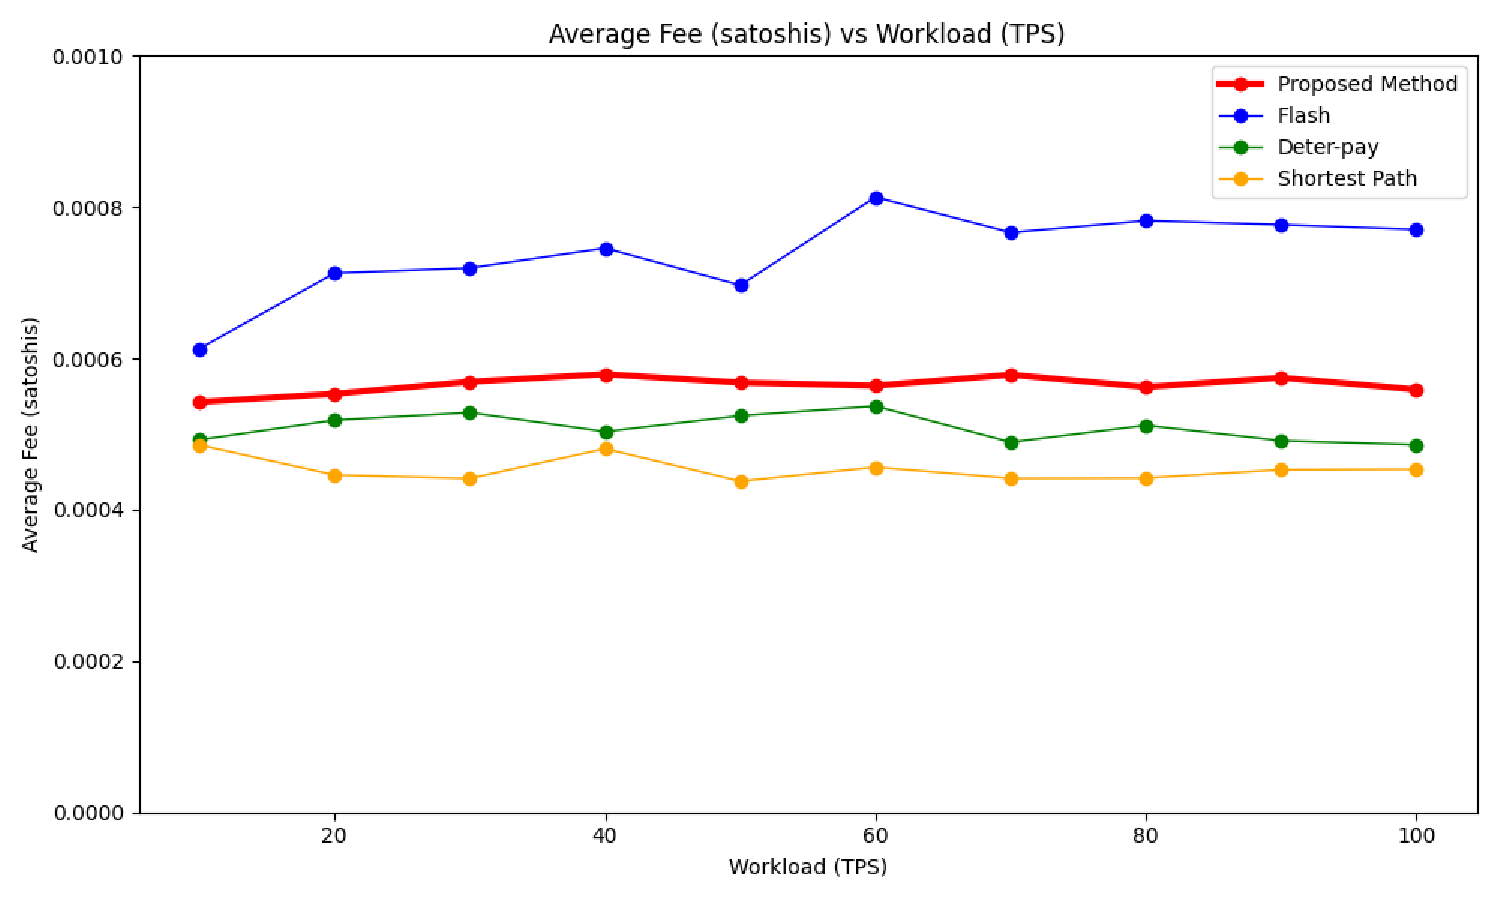
\includegraphics[width=\textwidth]{./figures/Transection_Fee.pdf}
        \caption{Transaction fees under different workloads.}
        \label{fig:Transection_Fee_TPS}
    \end{figure}

    
    Transaction Success Rate: Figure~\ref{fig:Success_rate_TPS} illustrates the variation in transaction success rate as the workload (TPS) increases. The proposed method consistently outperforms other protocols, including Deter-Pay, Flash, and Shortest Path, with all tested workloads. The method achieves the highest success rate even at a transaction frequency of 100 TPS and demonstrates its efficiency under high-load conditions. In contrast, Deter-Pay and Flash exhibit fluctuating or declining success rates as the workload increases, and Shortest Path consistently has the lowest performance among all evaluated methods.

    Transaction Latency: Figure~\ref{fig:Excution_time_TPS} displays the variation in transaction delay with different transaction workload frequencies. Compared to Deter-Pay and Flash, the proposed method exhibits stable and comparatively lower execution times. Shortest Path that depends solely on the most basic shortest path algorithm based on network topology, achieves the highest execution efficiency. The proposed method employs a two-phase payment process. A successful first payment phase can reduce overall transaction delay. Deter-Pay's requirement for path probing and channel reservation contributes to its higher transaction delay, especially as higher transaction frequencies may necessitate multiple probing and reservation attempts. Flash exhibits lower latency than Deter-Pay, but the method may incur higher delays due to repeated attempts. Flash lacks effective adaptation because of prior failures.

    Transaction Fees: Figure~\ref{fig:Transection_Fee_TPS} illustrates the variation in transaction fees under different transaction workloads. The proposed method incurs slightly higher fees than Deter-Pay but demonstrates a significant fee advantage over Flash. Shortest Path consistently yields the lowest transaction fees. The result is attributed to its reliance on a single path and a short hop count.

    
\section{Performance with Scaled Capacities}


    
\label{sec:performance_scaled_capacities}
    Currently, the average channel capacity of the Lightning Network is approximately 900,000 Satoshis. As off-chain payments become more widespread and more PCNs are practically deployed, channel capacities are expected to increase. This experiment was conducted to verify the effectiveness of the proposed method in the future development of payment channels. The simulation was examined with channel capacities scaled from one-fold to tenfold. These simulations were performed with a fixed testing duration and a constant transaction frequency.

    \begin{figure}[htbp]
        \centering
        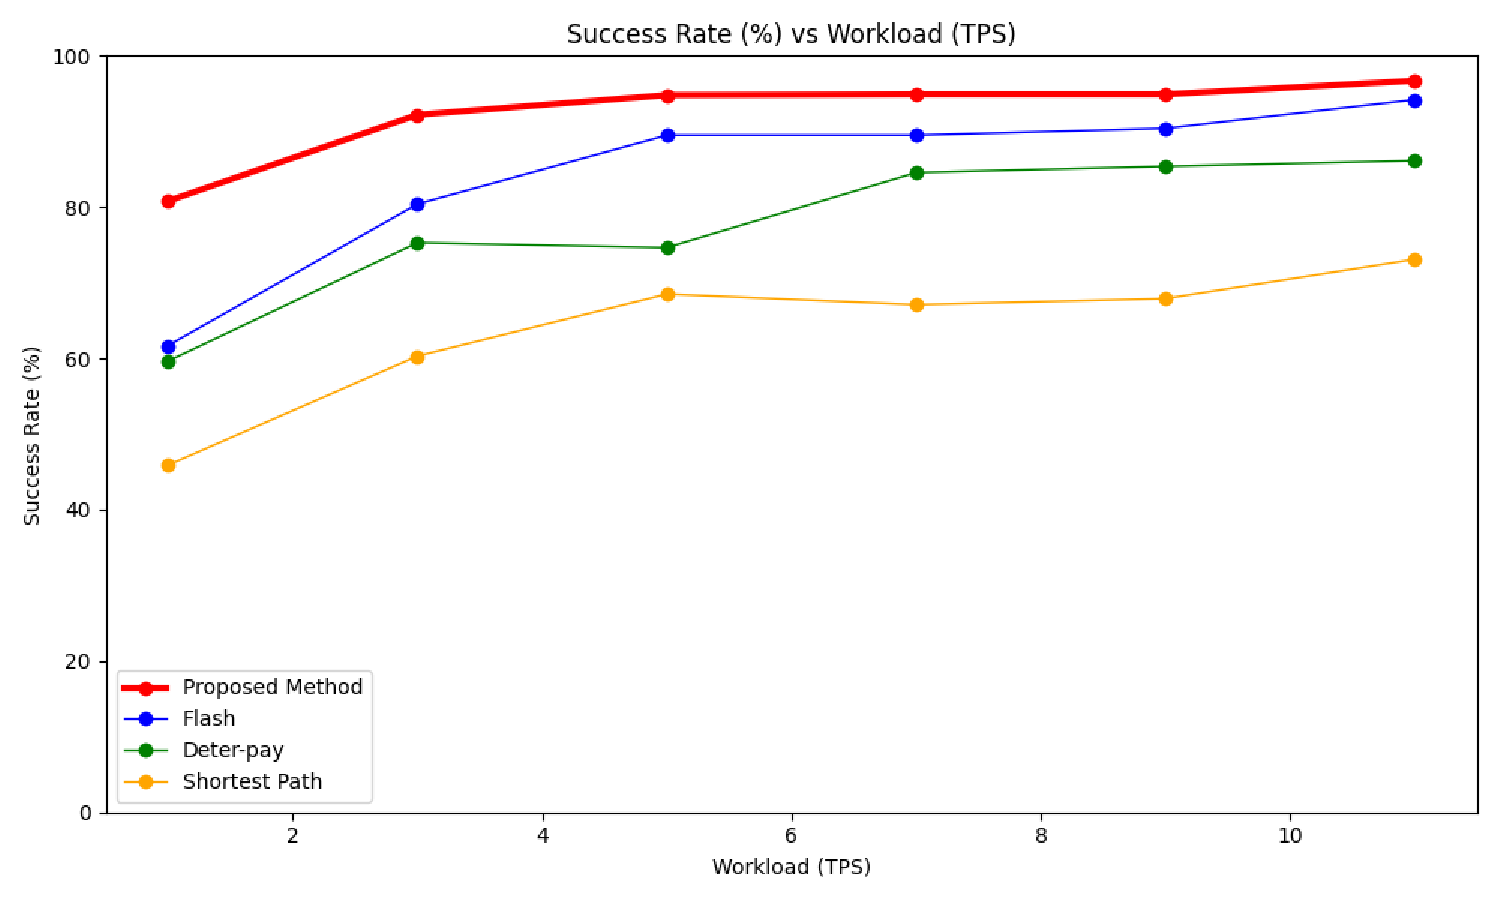
\includegraphics[width=\textwidth]{./figures/Success_rate_diff_channelsize.pdf}
        \caption{Success rate under different channel sizes.}
        \label{fig:Success_rate__diff_channelsize}
    \end{figure}
    
    \begin{figure}[htbp]
        \centering
        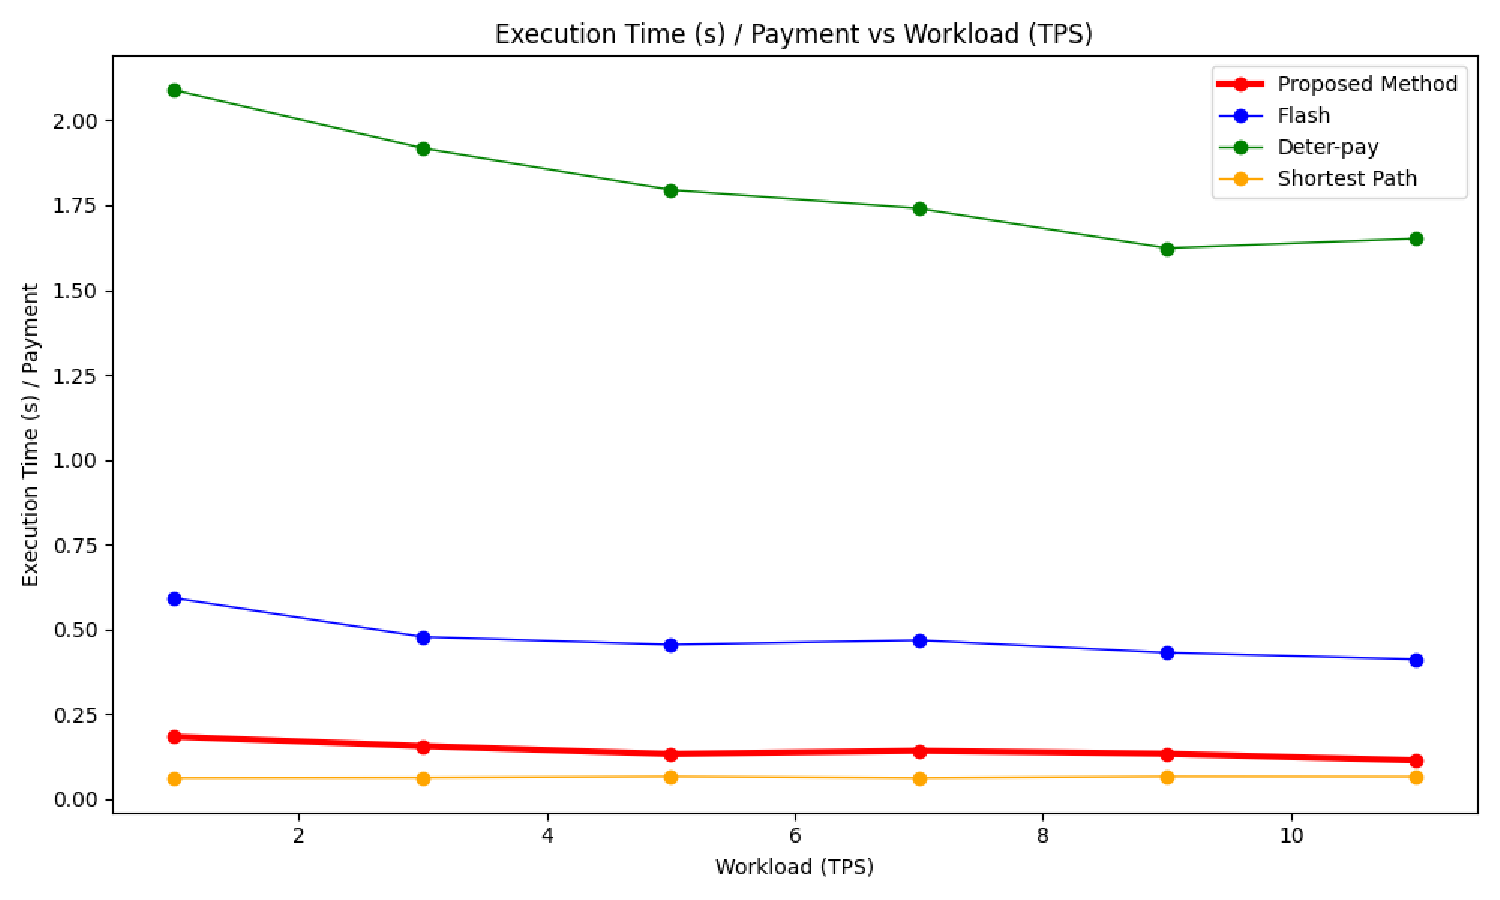
\includegraphics[width=\textwidth]{./figures/Excution_time_diff_channelsize.pdf}
        \caption{Execution time under different channel sizes.}
        \label{fig:Excution_time__diff_channelsize}
    \end{figure}
    
    \begin{figure}[htbp]
        \centering
        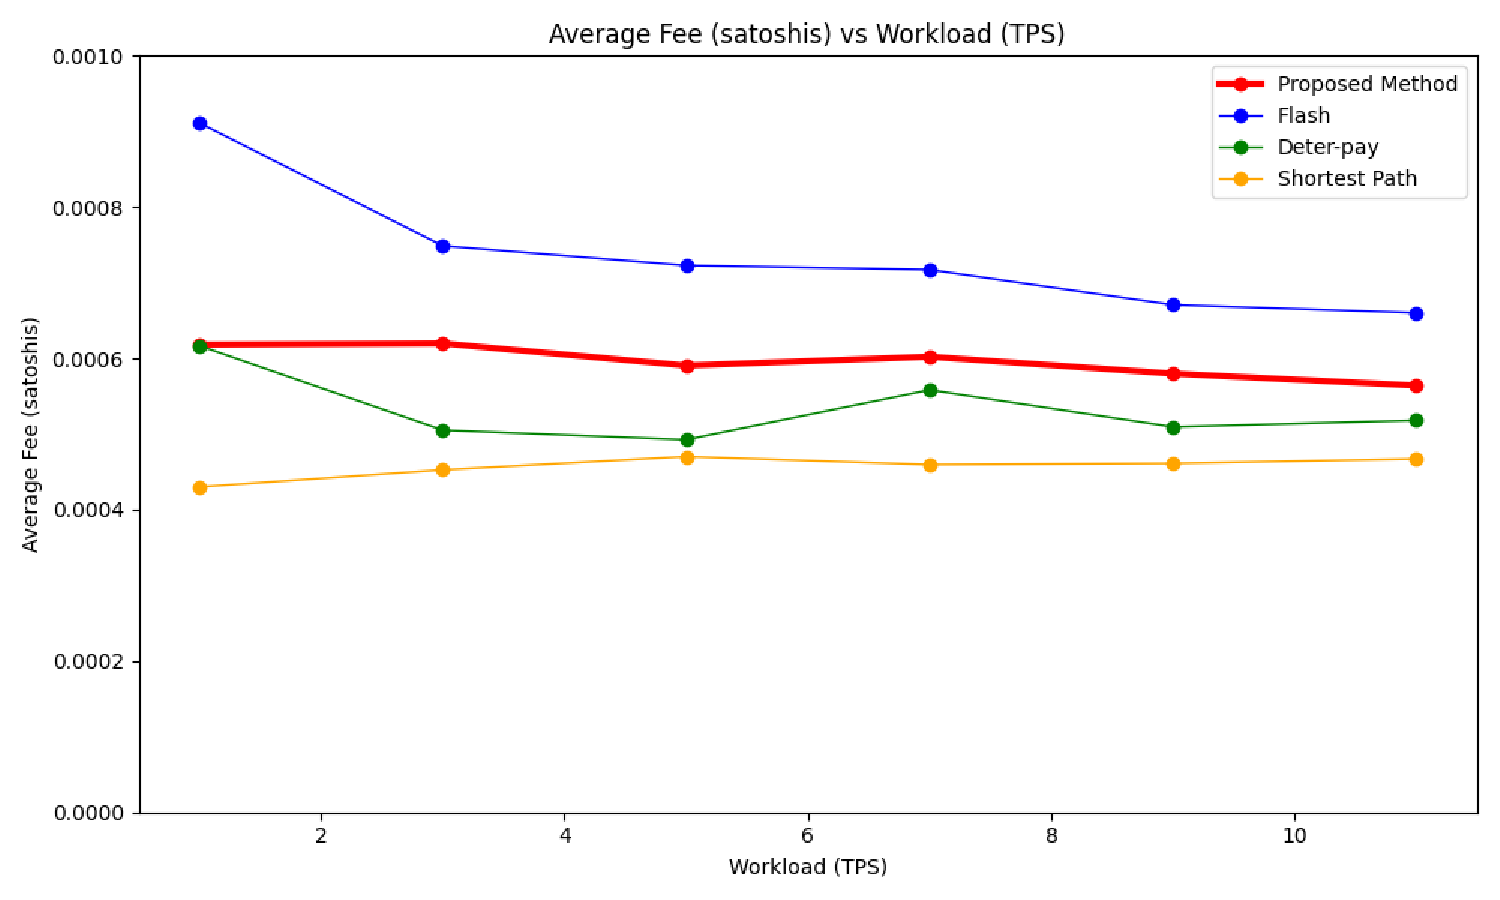
\includegraphics[width=\textwidth]{./figures/Transection_Fee_diff_channelsize.pdf}
        \caption{Transaction fees under different channel sizes.}
        \label{fig:Transection_Fee__diff_channelsize}
    \end{figure}

    Figure~\ref{fig:Success_rate__diff_channelsize} illustrates that the transaction success rates of all routing methods increase with the enhancement of channel capacity. Under conditions of increased channel capacity, the proposed method demonstrates a significant lead over Deter-Pay and Shortest Path methods.

    Figure~\ref{fig:Excution_time__diff_channelsize} indicates a gradual reduction in the execution time of the proposed method as channel capacity increases. This reduction is attributed to the increased likelihood of successful transactions in the algorithm's first payment phase with the larger channel capacity. Path score calculation and transaction splitting are used to achieve this success. This approach reduces the need for second-stage failed handling and consequently lowers transaction delay. In terms of transaction delay, the algorithm exhibits a more significant advantage compared to Deter-Pay and Flash.
    
    Finally, regarding transaction fees, Figure~\ref{fig:Transection_Fee__diff_channelsize} shows that the proposed method offers a lower fee advantage compared to Flash. Although its fees are higher than those of Deter-Pay and Shortest Path, the method demonstrates a significant advantage in success rate. The algorithm effectively balances success rate, execution time, and transaction fees.
    
\section{Performance with Failed Handling Mechanisms}

    The experiment was designed to verify the effectiveness of the algorithm's second phase, called Phase II: Failed Handling. The experiments with or without Phase II were conducted. The results were subsequently tested under different Capacity Scales.
    
    \begin{figure}[tb] 
        \centering
        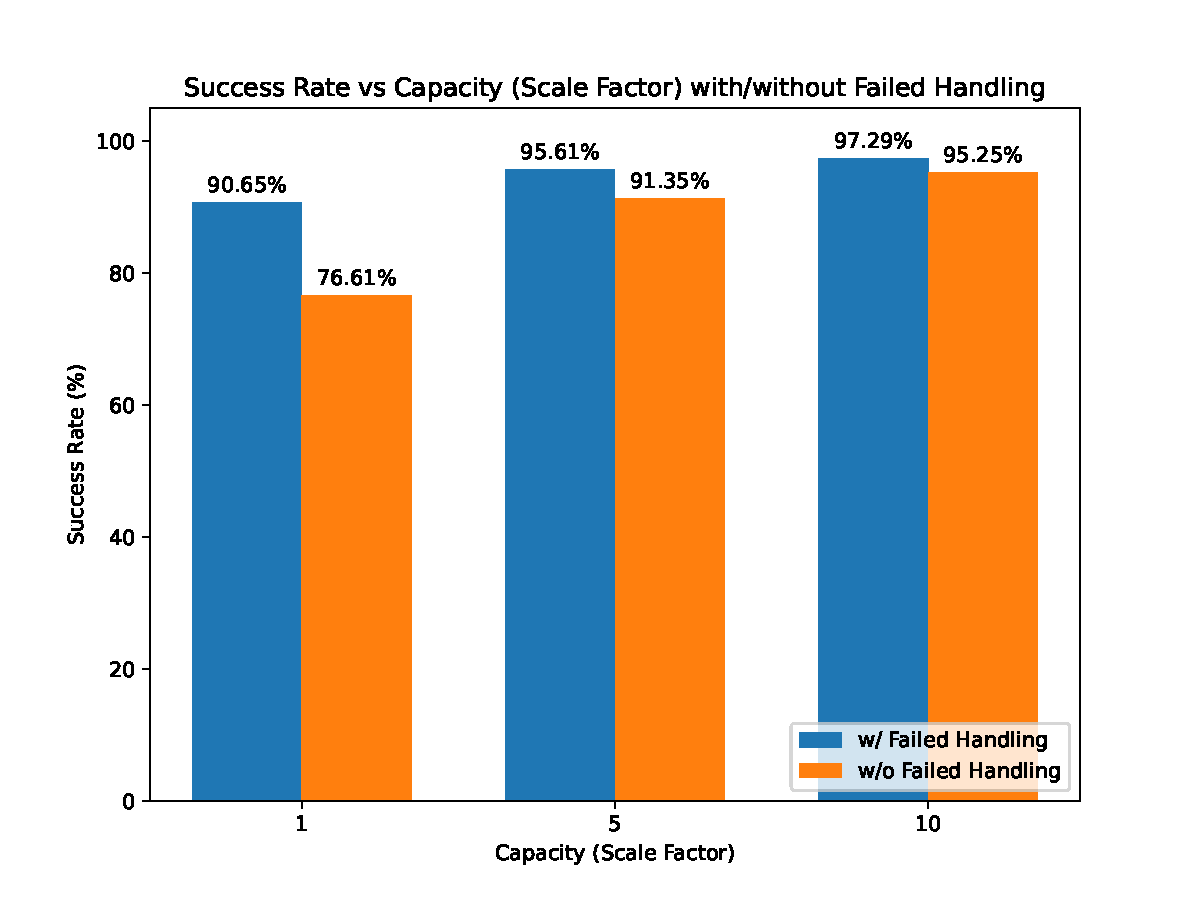
\includegraphics[width=\textwidth]{./figures/success_rate_w_wo_fail.pdf} 
        \caption{Success rate with and without failed handling mechanisms.} 
        \label{fig:success_rate_w_wo_fail}
    \end{figure}
    
    \begin{figure}[tb]
        \centering
        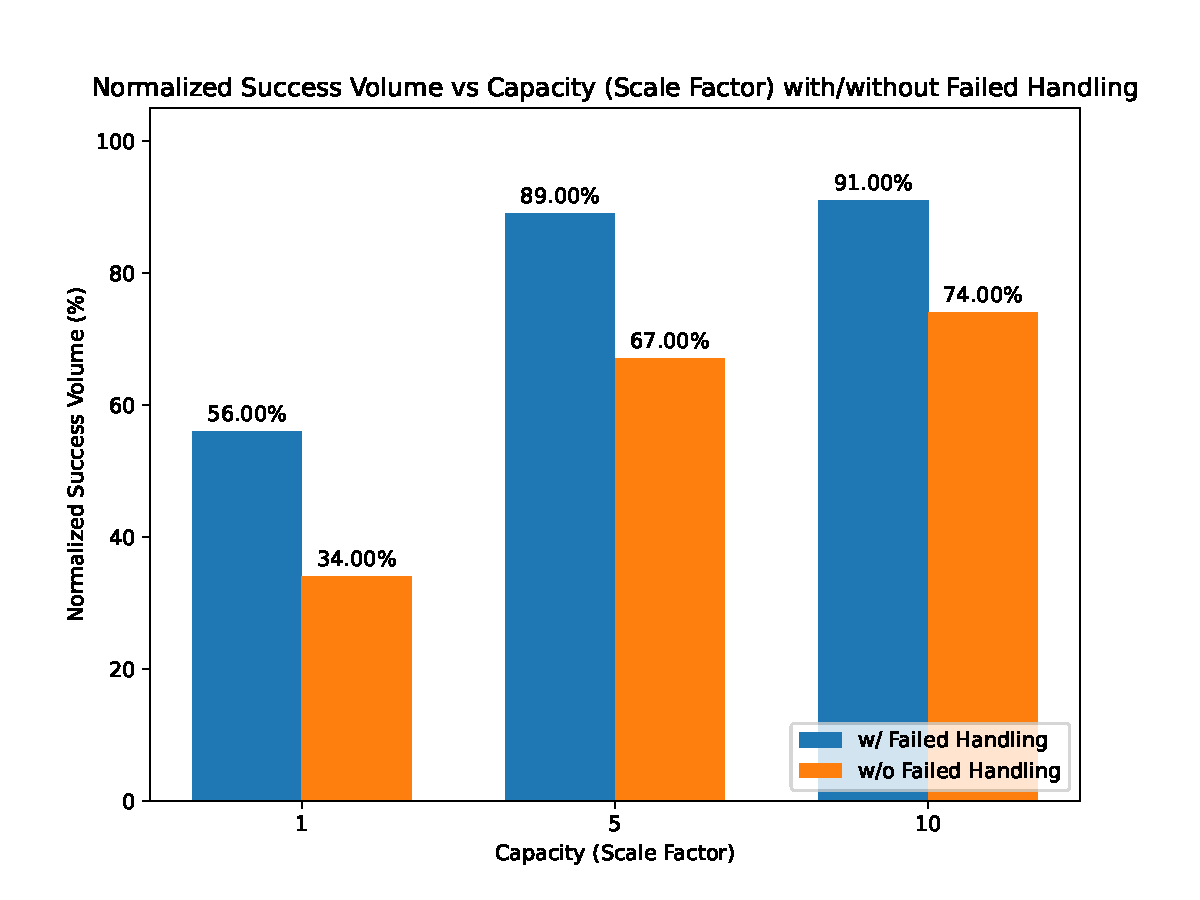
\includegraphics[width=\textwidth]{./figures/success_vol_w_wo_fail.pdf} 
        \caption{Successful volume with and without failed handling mechanisms.}
        \label{fig:success_vol_w_wo_fail}
    \end{figure}
    
    Figure~\ref{fig:success_rate_w_wo_fail} reveals that under smaller channel capacity scale factors, the Phase II: Failed Handling mechanism significantly enhances the transaction success rate. When channel capacity is larger, the improvement in success rate by failed handling becomes less prominent. Most transactions can be completed in the first phase. This experimental result corroborates the findings in Section~\ref{sec:performance_scaled_capacities} regarding lower transaction delay with larger channel capacity. This outcome is similarly attributed to the increased success rate in the first phase.

    Figure~\ref{fig:success_vol_w_wo_fail} demonstrates a significant increase in the total successful transaction volume ratio regardless of the channel capacity. The Phase II failed handling method effectively satisfies large transaction demands and enhances transaction completion rates. The results are achieved by enabling re-attempts based on probing results and intelligently allocating large transaction amounts to available channels.

%------------------------- Conclusion and Future Works -------------------------%
\chapter{Conclusion and Future Work} \label{Chap:Conclusion}

\section{Conclusion}

    This thesis presents a two-phase routing algorithm to improve efficiency and reliability in PCNs. The algorithm consists of an initial payment attempt and a re-exploration phase triggered upon failure. Adaptive responses can be enabled to dynamic or inconsistent network conditions.
    
    Routing decisions are informed by a combination of factors, including channel capacity, balance status, fee conditions, and usage patterns. The integrated approach improves path selection, reduces payment failure rates, and lowers overall transaction costs.
    
    Routing performance was examined based on the simulated transaction workloads and network conditions. The proposed algorithm typically outperforms existing methods in terms of success rate, latency, and cost. The evaluation results confirm the effectiveness of the algorithm for scalable PCN routing.

\section{Future Work}
	
    In this research, it is assumed that channel-related information can be obtained through trusted nodes. Nevertheless, considering the high demands for privacy protection in decentralized platforms, it is imperative that no sensitive data is compromised through any means. Therefore, future work ought to explore the development of more efficient routing mechanisms and also guarantee the privacy of every node.
	
}\end{thesis}


%------------------------- References -------------------------%
\singlespace {\large
\bibliography{Reference}
}
\bibliographystyle{IEEEtran}

\doublespace

%--------------------------------------------------------%

\end{document}


